\documentclass[12pt,letter paper]{article}
\usepackage[margin=1in]{geometry}
\usepackage{setspace} 
\usepackage{natbib}
\usepackage{gensymb}
\usepackage[utf8]{inputenc}
\usepackage{amsmath} 
\usepackage{multirow}
\usepackage{enumitem}
\usepackage{mathtools}
\usepackage{amssymb}
\usepackage[utf8]{inputenc}
\usepackage[english]{babel} 
\usepackage{amsthm}
\usepackage{graphicx}
\usepackage{float}
\usepackage{natbib}
\usepackage{setspace}
\usepackage{qtree}
\usepackage{dsfont}
\usepackage{array}
\usepackage{longtable}
\usepackage{chngcntr}
\newcolumntype{P}[1]{>{\centering\arraybackslash}p{#1}}
\newtheorem{theorem}{Theorem}[section]
\newtheorem{corollary}{Corollary}[theorem]
\newtheorem{lemma}[theorem]{Lemma}
\newtheorem{axiom}{Axiom}[subsection]
\newtheorem{proposition}{Proposition}[subsection]
\newtheorem{fact}{Fact}[subsection]
\newtheorem{exercise}{Exercise}[section]
\newcommand{\R}{\mathbb{R}}
\newcommand{\N}{\mathbb{N}}
\newcommand{\Z}{\mathbb{Z}}
\newcommand{\Q}{\mathbb{Q}}
\newcommand{\C}{\mathbb{C}}
\newcommand{\Hamilton}{\mathbb{H}}
% !TeX spellcheck = en_GB 
\newcommand\myeq{\mathrel{\stackrel{\makebox[0pt]{\mbox{\normalfont\tiny $\infty$}}}{\sim}}}
\title{Member and Customer Responses to Demand Shifters in Bicycle Share Programs}
\author{Liam MacDonald}
\doublespacing
\begin{document}
\maketitle
\begin{abstract}
The goal of this paper is to determine the factors that influence the demand for bicycle share programs and whether they differ between members and customers.  The factors being investigated include a number of weather variables, the day of the week and air quality.  The empirical approach uses a fixed effects model with an instrumental variable for air quality to determine the causal effect of each variable and identify how they differ across two groups of users.  Trip data from bicycle share programs is available in many cities across the United States, and this paper leverages 7 major cities to estimate the model.  The results show that temperature, rain, snow and day of week are the significant drivers and all affect customers significantly more than members who subscribe to the service.
\end{abstract}



\section{Introduction}

The environmental impact of an industry has become an important topic of conversation in recent years and has resulted in significant research and investment into how we can expand the economy with as little environmental damage as possible.  Transportation is one industry that has a particularly large environmental impact and thus has been at the forefront of this conversation.  Many advancements have been made to reduce the emissions created from the movement of people, from electric cars to improvements in public transportation systems which allow more people to travel faster with less environmental impact.  A large part of reducing the environmental impact of commuting has been the promotion of bicycle use as a form of transportation.  Things like separated bicycle lanes or bicycle pathways have increased safety and convenience thereby increasing the number of people who substitute away from less environmentally friendly forms of transportation. \\

A new development that has become more common as a way to increase the amount of bicycles being ridden is bicycle share programs.  Many cities have adopted a docked bicycle share program to increase the use of bicycles as a form of transportation and supplement the use of existing transportation services.  These programs operate using a network of bicycles and docking stations which allow short term rentals to commute from one area of a city to another.  The relatively low cost compared to other forms of transportation as well as the convenience compared to walking or using your own bike make these programs an attractive tool in commuting for many people.  Most major cities in the United States and Canada now have some form of bicycle share program and many smaller programs exist within certain neighbourhoods of a city or on university campuses. \\

In order to use these services customers are charged for every trip or can choose to buy a daily, monthly or annual pass which allows for unlimited trips in the given time period.  In most scenarios a trip consists of a 30 minute ride, if the bike is not docked within the 30 minutes a fixed rate per extra half hour is charged.  There is slight variations to each system, for example the Bluebikes program in Boston offers 30 minute one time trips but the monthly and annual memberships allow trips up to 45 minutes and the daily pass allows trips up to 2 hours.  Table A.1 in the Appendix gives pricing and trip length information for each bicycle share program discussed in this paper.  The common thread across these programs is there exists different payment options which allow either one time use, daily use or a longer subscription, which will be the focus of the analysis. \\



As the popularity of these programs continues to grow, many of the companies behind implementing them tout the potential benefits.  The common arguments made in favour of these programs include: increased exercise, lower congestion, increased multimodal transportation and numerous environmental benefits.  However, most of the claims are made with relatively little evidence to support them.  More advanced research is required in order to understand the true impact and how to maximize effectiveness moving forward. \\

Figure 1 shows the number of customer and member trips each year in 7 cities along with the standard deviation.  This first thing to note is the average trips by members are significantly higher but more importantly we can see from this graph that customer trips have a much higher variance relative to the mean.  This shows support for the hypothesis that members respond to factors influencing rides differently then customers.  Less variance among rides means that on any given day a member is less likely to forgo a ride for any reason.  The graph provides a valuable insight but does not give us any indication of what causes customers or members to forgo trips. \\
\begin{figure}[H]
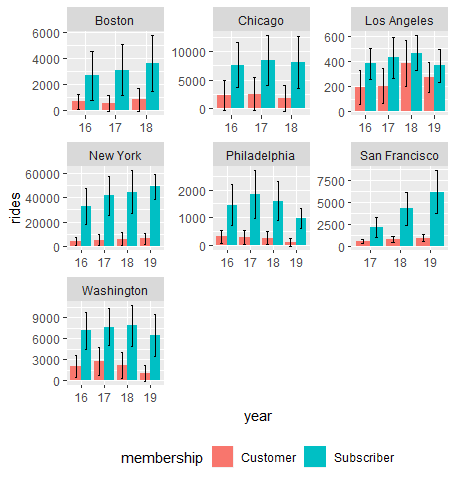
\includegraphics[scale=1]{plot_1.png}
\caption{Number of Trips By City and Membership Type}
\end{figure}

There has been a growing literature trying to understand exactly who is using these bicycle share programs and what drives demand for them (\cite{fishman2013bike}, \cite{el2017effects}, \cite{mattson2017bike}).  Much of the research to date has shown that demand is largely driven by weather variables such as wind, precipitation and temperature; other key determinants include bicycle infrastructure, the presence of college campuses, convenience of stations and cost.  The common measurement of demand in the existing literature is either the number of trips per day or the number of trips per bike per day.  However, \cite{fishman2015factors} uses a different approach to identify the factors that affect bike share membership by looking at some of the relatively less successful programs in Australia.  My paper will add to this literature by connecting these two ideas.  The goal of this paper is to identify the differences in how factors affect demand for one time and daily users (customers) as oppose to monthly or annual subscribers(members), where demand is defined as rides per day.  The variables of interest in this case are weather variables which have been identified as driving factors of demand and will include additional variables not discussed in previous literature such as air quality and day of week variables.  \\





\section{Literature Review}

How weather and outdoor conditions affects the use of transportation has been the focus of a large body of research.  \cite{bocker2013impact} presents a synthesis of the literature finding that weather conditions have significant impact on active forms of transportation and outdoor activities which are the two broad uses of bicycle share programs.  Some of this literature extends to include some demographic comparisons such as \cite{saneinejad2012modelling} which finds that younger people and women are more sensitive to weather changes such as temperature and rain.  To my knowledge there is no existing literature which investigates how these factors affect members and customers differently. \\


Thus far I have discussed much of the existing literature on active transportation and bicycle share programs that is relevant to my topic but none of this research addresses membership influences specifically.  However, how people decide between memberships and one time passes has been investigated in previous economic literature.  \cite{dellavigna2006paying} performed a novel analysis to show that many people who purchase memberships are overly optimistic about their use and would experience significant cost savings by buying one time entry fees or a group of entry fees.  This paper uses data from health clubs which tracks the amount of times a member uses the gym.  The context of the paper is slightly different but the results are relevant.  There is not a direct comparison to the use of health clubs by customers but the fact that members are under utilizing them is weak evidence to suggest that people do not consider the subscription fee paid when they are making decisions.  Based on the results of this paper, we might expect that there would not be significant differences in the way members and customers respond to factors affecting demand.  

If we believe the story explained in the previous paragraph, then the expectation is that members are not more likely to use bicycle share programs because they have paid a fee and will respond similarly to different factors.  Some research has tried to examine these topics in the setting of bicycle share programs.  Specifically, \cite{lathia2012measuring} attempt to identify some of the changes in usage in London's bicycle share program after a policy increasing ease of access for ``casual" users was implemented.  The results show that the change allowing users to access bikes with only a debit card and no application process increased weekend use as well as use at specific stations.  This shows preliminary evidence for the idea that customers and members use the service differently and therefore will be affected differently by certain factors.   \\

In existing literature the topics of bicycle share usage and membership have both been discussed at length.  My paper adds to the literature by specifically addressing how customers and members operate differently in the context of bicycle sharing.  There is still uncertainty about the most effective form of payment plan especially with respect to the consumer decision.  Understanding what types of users are using the bikes and how they respond factors can have implications for pricing, station placement and bicycle redistribution making it a valuable insight for policy makers and bicycle share businesses alike. 


\section{Empirical Model}

The empirical approach in this paper is adapted from \cite{deryungina2016mortality} which estimates the effect of air quality on mortality in elderly populations in the United States.  This is the ideal approach for the context of our data because of the need to instrument air quality, an endogenous regressor, in multiple cities.  As they note in their paper many instruments for air quality are specific to a certain context and cannot be generalized to use across multiple regions or cities.  However, using research from the EPA that suggests air quality in a specific area is significantly impacted by particulates carried by wind; \cite{deryungina2016mortality} identifies wind direction as a valid instrument for PM 2.5 concentration.  Although my paper is investigating a different field than discussed in \cite{deryungina2016mortality} the empirical strategy is valid for this setting as well.  By using wind direction in each city, air quality can be predicted in a way that is exogenous to the use of bicycles and therefore we can obtain a causal estimate of the effect of air quality on bicycles.  \\



The instrumental variable regression model will be estimated using two stage least squares to account for the endogeneity of the air quality variable.  All other variables are assumed to be exogenous, which seems reasonable as they are determined by natural phenomena.  Since the data set is a panel data set which includes seven cities in the United States, the model will use city-month fixed effects to remove the impact of any seasonal changes in bicycle use or any differences that exist among cities caused by infrastructure or any other fixed attribute of the city.  Therefore the first stage equation can be written as
\begin{gather*}
PM_{it} = \sum_{i = 1}^7 \sum_{j = 1}^4 WD_{ijt} + X_{it}\beta + \delta_{mi}  + \epsilon_{it}
\end{gather*}
where $PM_{it}$ is the PM 2.5 concentration, $X_{it}$ represents other controls for weather and day of the week and $\epsilon_{it}$ is the error term in city $i$ on date $t$.  The $\delta_{mi}$ represents city-month fixed effects which are included to reduce bias from seasonal changes which may influence rides taken.  The variable $WD_{ijt}$ is a dummy variable for four 90 degree intervals of wind direction, represented by $j$, in city $i$ on date $t$ which will act as the main instrumental variable in the regression.  Wind direction here is an effective instrument since it is unlikely that any cyclists make decisions to ride or not based on the direction of the wind and therefore the exogeneity assumption is satisfied.  As discussed previously, there is existing literature which shows that wind direction effectively predicts particulate matter concentration; both the assumptions required for an instrumental variable are satisfied.  The first stage equations are included in the appendix and show that many of the effects of wind direction are significant on air quality and have relatively high R-squared (0.38 for the fixed effects model) meaning it is unlikely we have a weak instruments problem.  The second stage equation is given by
\begin{gather*}
Y_{it} = \widehat{PM}_{it} + X_{it}\beta + \delta_m + \gamma_i + u_{it}
\end{gather*}
where $Y_{it}$ is the log number of rides, $\widehat{PM}_{it}$ is the predicted PM 2.5 concentration from the first stage, $u_{it}$ is the error term and all other variables are the same as the first stage.  These two equations will be estimated aggregated by total number of trips taken in the city, then estimated separately using the total number of trips taken by members and total number of trips taken by customers as the dependent variable.  The first estimation will allow us to identify the total change in the number of riders caused by each dependent variable, while the next two can be used to compare how each group of riders is affected differently.  


\section{Data and Summary Statistics}

\subsection{Bicycle Share Usage Data}
The first thing we need to estimate the empirical specification mentioned above is data on the number of rides taken in a city by both member and customers in a given city.  The data for many companies operating bicycle share programs is publicly available through their websites.  This paper will investigate 7 cities in the United States dating back to 2016 including: Chicago, New York, San Francisco, Los Angeles, Philadelphia, Boston and Washington.  There is data available for many other cities but this sample comprises most of the rides taken in the United States over the time period.  There is no gaps in the data for any of the cities other than San Francisco which did not have a bicycle share program until midway through 2017 and Los Angeles which did not have a bicycle share program until midway through 2016.  \\

The data sets for all cities include data on the following variables for each trip: start time, end time, start station, end station, bike id, duration and whether or not they are a member or customer.  With some cities including additional data on the location of each start and end station and some personal characteristics such as gender and birth year.  Since the variable of interest for this paper is the amount of trips in a day and all data sets include start time and end time the aggregated number of trips can be calculated from the data in all cities.  All trips that are less than 60 seconds have been removed from the data sets by the publishers as they may result in error as well as all service and test trips taken by staff.

\subsection{Weather Data}
As discussed previously weather has been identified as one of the driving factors of bicycle share demand.  Detailed daily weather data is available from the National Oceanic and Atmospheric Administration's National Centers for Environmental Information.  The data used in this analysis is collected from land base stations, the relevant variables for this analysis include temperature, rain, snow, snow depth, wind speed and wind direction.  All the data is collected in imperial measurements but it has been converted to metric for the analysis.  This data is available at the daily level for all cities, however some observations are dropped due to missing data from either temperature or wind direction which was not recorded for the day.  

\subsection{Air Quality Data}
Air quality data is available at the city level from the Environmental Protection Agency for a number of different air pollutants.  For the cities in the sample Los Angeles, San Francisco and Philadelphia have daily data, and the remaining four cities have data available every 3rd day.  The pollutant of interest in this case is PM 2.5, which represents particulate matter less than 2.5 mm in size present in the air and is measure micrograms per meter cubed ($\mu g /m^3$).  PM 2.5 concentration is one of the most commonly discussed air quality measures as it is often associated with some of the most dangerous air quality conditions for humans.  Due to the small size of the particles they can remain in the air longer and have damaging effects when inhaled by humans.  In addition, high concentrations can make for more difficult exercise conditions potentially affecting the use of active forms of transportation.  




\subsection{Summary Statistics}
The mean and standard deviation for all the relevant variables broken down by city is presented in Table 1 below.  There is a number of different advantages to working with the data presented below.  First of all, since so much of the data required is publicly available it is possible to obtain a high volume of data, helping to increase the fit of the model.  We can also see from Table 2 that our dependent variable has a large amount of variation, with standard deviations close to the same level as the mean.  With this large amount of variation in the dependent variable, factors affecting the number of trips will be more likely to show significance in a regression.  In addition, we can see from Table 1 that there is a variety of different environments we are investigating.  Since, each city represents a different climate, including multiple cities allows more variation in our independent variables.  For example, Boston will include a number of cold, windy days with high precipitation while LA will mostly consist of exceptionally hot dry days.  The increased variation across the variables allows for much greater power in the results.\\



One problem may be the relatively low estimates for air quality.  The World Health Organization recommends keeping average annual PM 2.5 levels below 10 $\mu g / m^3$, which we can see from Table 1 is met by 5 out of 7 cities and both LA and San Francisco are very close to the target.  Furthermore, other than San Francisco the standard deviation relative to the mean is fairly low, meaning there is a lack of observations with high levels of PM 2.5.  We can see this further in the summary statistics presented in the appendix which show the 75th percentile of PM 2.5 in this data set is only 12.2, which is fairly close to the target annual average.  The lack of poor air quality in the data means it is unlikely that air quality is a significant driver of behind the decision to use ride share services.  \\


\begin{table}[!htbp] \centering 
  
  \label{} 
\begin{tabular}{ lccccccc} 
\\[-1.8ex]\hline 
\hline \\[-1.8ex] 
City & Boston & Chicago & LA & NY & Philadelphia & San Fran & Washington \\ 
& & & & & & & \\
Mean & & & & & & & \\
\quad Temperature & 11.83 & 12.13 & 19.62 & 14.36 & 13.39 & 15.22 & 15.32 \\ 
\quad Rain & 0.34 & 0.24 & 0.11 & 0.36 & 0.31 & 0.14 & 0.25 \\ 
\quad Snow & 0.39 & 0.00 & 0.00 & 0.21 & 0.16 & 0.00 & 0.15 \\ 
\quad Snow Depth & 0.00 & 0.00 & 0.00 & 0.30 & 0.24 & 0.00 & 0.14 \\ 
\quad Wind Speed & 17.99 & 15.74 &  2.67 &  7.86 & 14.47 & 15.79 & 14.23 \\ 
\quad PM2.5 &  5.99 &  9.47 & 12.02 &  7.66 &  9.93 & 11.06 &  7.45 \\ 
\quad Customer Trips &  685.01 & 2211.99 &  273.71 & 5101.39 &  267.94 &  751.51 & 2182.99 \\ 
\quad Member Trips &  3084.86 &  7991.37 &   428.06 & 39912.49 &  1568.01 &  4065.18 &  7436.32 \\ 
 & & & & & & & \\
Standard Deviation & & & & & & & \\
\quad Temperature &  9.59 & 11.18 &  4.41 &  9.38 &  9.99 &  3.54 &  9.60 \\ 
\quad Rain & 0.80 & 0.64 & 0.55 & 0.83 & 0.83 & 0.55 & 0.69 \\ 
\quad Snow & 2.40 & 0.00 & 0.00 & 1.60 & 1.16 & 0.00 & 1.15 \\ 
\quad Snow Depth & 0.00 & 0.00 & 0.00 & 1.83 & 1.51 & 0.00 & 1.15 \\ 
\quad Wind Speed & 6.00 & 5.58 & 1.51 & 3.82 & 5.96 & 7.31 & 5.65 \\ 
\quad PM2.5 &  2.97 &  4.56 &  6.74 &  3.89 &  4.71 & 14.13 &  3.64 \\ 
\quad Customer Trips &  707.24 & 2593.72 &  177.44 & 4488.48 &  244.62 &  350.59 & 1840.87 \\ 
\quad Member Trips &  2012.01 &  4257.39 &   150.51 & 16548.38 &   779.09 &  2284.78 &  2784.13 \\ 
\hline \\[-1.8ex] 
\end{tabular} 
\caption{Summary Statistics for Variables Relevant to Analysis} 
\end{table} 




\section{Results}
Table 2 shows the aggregated results for the model discussed in the empirical strategy.  The first two models are OLS results and the other four instrument for PM 2.5.  Models 1,2,4 and 6 include city month fixed effects and models 2,4 and 6 cluster standard errors by city.  The main specification of interest is model 6 as it provides the best estimate of a causal relationship for each variable.  The dependent variable in this case is the log of the number of trips taken on date $t$ in city $i$.  We can see that most of the results are the direction we would expect.  The surprising results are the variables which have no effect on number of trips taken in the model, namely wind speed and air quality.  \\

The inclusion of air quality variables in this paper did not seem to have any impact on the number of rides taken other than model 3 which is the IV model with no fixed effects or clustering.  Since city clustering results in large increases in standard errors the significant result in model 3 should be mostly ignored.  A large issue with obtaining significance on air quality in this analysis is the lack of data available for days with extremely high levels of PM 2.5.  The WHO suggests that cities should aim to keep daily averages of PM 2.5 below 25 $\mu g /m^3$ to avoid adverse health affects.  We can see in Table A.4 the data set used there is only 88 observations which have a value higher than this recommendation and Boston, New York and Washington all have none.  Ideally we could look at days with extremely bad air quality compared to normal levels as this would be the most likely way air quality would have an effect on trips, unfortunately the data does not create this kind of natural experiment.  Since the data points with large PM 2.5 values are concentrated mostly in L.A. and San Francisco (see table A.4) we are forced to remove fixed effects to obtain estimates with any significant magnitude.  However, with our lack of city level controls, removing city fixed effects makes our estimates  largely meaningless. \\

Overall the results indicate that most trips are taken on weekdays where there is no rain.  Each additional centimeter of rain reduces the amount of trips on any given day by approximately 20\% while weekends have 28\% less trips then weekdays.  One of the most surprising results is that snow and snow depth have very little effect on the number of bicycle trips.  It is unlikely that the variation is being removed by fixed effects as their is not significant changes in the results when the fixed effects are not included in models 3 and 4.  It is more likely that the lack of large snowfalls on a regular basis in any of the cities results in too little variation to find a result, further the temperature variable may be picking up much of the drop in trips on days with snow.  Any day there is snow will also be very cold and it is unlikely that someone who would decide to take a bike on a day which is below zero would be deterred by a small amount of snow.  \\

Temperature also has interesting effects on the amount of trips taken.  As we would expect higher temperatures correspond to more trips taken, where  each degree higher adds approximately 4 percent more trips each day, a fairly large number when we consider temperature could swing over 20 degrees in the data set.  The above $28^{\degree}$C variable indicates that extremely high temperature days are the most popular to use these services, however when it is over $28^{\degree}$C the number of trips starts decline as temperature increases.  Again this is what we would expect, as temperatures start to get extremely high it becomes less pleasant to bike and reduces the number of trips.
\bgroup
\def\arraystretch{0.5}
\begin{table}[H]
\begin{center}
\begin{tabular}{l c c c c c c }
\hline
 Variables & Model 1 & Model 2 & Model 3 & Model 4 & Model 5 & Model 6 \\
\hline
Wind Speed              & $-0.01^{***}$ & $-0.01^{**}$  & $-0.01$       & $-0.01$       & $-0.00$       & $-0.00$       \\
                        & $(0.00)$      & $(0.00)$      & $(0.01)$      & $(0.10)$      & $(0.00)$      & $(0.00)$      \\
Rain                    & $-0.21^{***}$ & $-0.21^{***}$ & $-0.26^{***}$ & $-0.26^{***}$ & $-0.20^{***}$ & $-0.20^{***}$ \\
                        & $(0.01)$      & $(0.02)$      & $(0.04)$      & $(0.07)$      & $(0.01)$      & $(0.02)$      \\
Snow                    & $-0.06^{***}$ & $-0.06^{***}$ & $-0.08^{**}$  & $-0.08^{*}$   & $-0.06^{***}$ & $-0.06^{***}$ \\
                        & $(0.00)$      & $(0.01)$      & $(0.03)$      & $(0.04)$      & $(0.00)$      & $(0.01)$      \\
Snow Depth              & $-0.09^{***}$ & $-0.09^{***}$ & $-0.03$       & $-0.03$       & $-0.09^{***}$ & $-0.09^{***}$ \\
                        & $(0.00)$      & $(0.02)$      & $(0.02)$      & $(0.10)$      & $(0.00)$      & $(0.02)$      \\
Weekend                 & $-0.28^{***}$ & $-0.28^{***}$ & $-0.31^{***}$ & $-0.31^{*}$   & $-0.28^{***}$ & $-0.28^{***}$ \\
                        & $(0.01)$      & $(0.08)$      & $(0.06)$      & $(0.12)$      & $(0.01)$      & $(0.08)$      \\
Above $28^{\degree}$C                & $2.25^{***}$  & $2.25^{***}$  & $1.88$        & $1.88$        & $2.36^{***}$  & $2.36^{***}$  \\
                        & $(0.67)$      & $(0.48)$      & $(4.00)$      & $(4.89)$      & $(0.69)$      & $(0.55)$      \\
Temperature             & $0.04^{***}$  & $0.04^{***}$  & $0.03^{***}$  & $0.03^{*}$    & $0.04^{***}$  & $0.04^{***}$  \\
                        & $(0.00)$      & $(0.00)$      & $(0.00)$      & $(0.01)$      & $(0.00)$      & $(0.00)$      \\
PM2.5                   & $-0.00^{*}$   & $-0.00$       & $-0.18^{***}$ & $-0.18$       & $0.00$        & $0.00$        \\
                        & $(0.00)$      & $(0.00)$      & $(0.02)$      & $(0.21)$      & $(0.01)$      & $(0.01)$      \\
Above $28^{\degree}$C*Temperature    & $-0.09^{***}$ & $-0.09^{***}$ & $-0.04$       & $-0.04$       & $-0.09^{***}$ & $-0.09^{***}$ \\
                        & $(0.02)$      & $(0.02)$      & $(0.14)$      & $(0.18)$      & $(0.02)$      & $(0.02)$      \\
Constant                &               &               & $9.41^{***}$  & $9.41^{**}$   &               &               \\
                        &               &               & $(0.23)$      & $(3.36)$      &               &               \\
\hline
Num. obs.               & 3974          & 3974          & 3974          & 3974          & 3974          & 3974          \\
R$^2$       & 0.96          & 0.96          & -0.65         & -0.65         & 0.96          & 0.96          \\
Adj. R$^2$  & 0.96          & 0.96          & -0.65         & -0.65         & 0.96          & 0.96          \\
Model & OLS & OLS & IV & IV & IV & IV \\
Fixed Effects & city-month & city-month & none & none & city-month & city-month \\
Clustered S.E. & none & city & none & city & none & city \\
\hline
\multicolumn{7}{l}{\scriptsize{$^{***}p<0.001$, $^{**}p<0.01$, $^*p<0.05$}}
\end{tabular}
\caption{Results for log trips where trips includes both customers and subscribers}
\label{table:coefficients}
\end{center}
\end{table}
\egroup

Overall Table 2 provides interesting insights into how ridership changes across days but provides limited information that could be used by policy makers and companies to improve the service.  Table 3 presents the main results which compare all the coefficients from Table 2 across members and customers.  The top panel of the table labeled``Customers" gives the coefficient estimates for all variables on log number of trips for customers only.  The bottom panel labeled ``Member Deviations" provides the difference between the coefficient estimates for members and the coefficient estimates for customers.  Therefore, any variable which shows significant effects in the bottom panel of Table 3 can be said to have a different effect for members and customers.  \\

PM 2.5 concentration again only shows significant results when looking at an IV model with no fixed effects or clustering.  The members trips are significantly less affected then the customers in the model but as in the aggregated result there is not much we can say due to the lack of observations with measures of poor air quality in the data set.  The inclusion of city month fixed effects removes this variation and causes the estimates to return to 0.  While this may be the case and air quality is actually the cause of these results is uncertain as there could be other reasons in those peak air quality events which is driving change in a particular city.  The data set does not have enough variation to determine these results in the fixed effects model and therefore there is not much we can say about the way air quality affects trips.  One encouraging result is in the model with no fixed effects even if a factor other than air quality is biasing the results, it affects members to a lesser degree as we would expect to see.   \\


One of the most interesting results in this case is the weekend variable, which shows that customers take significantly more trips on weekends.  We know that previous research has shown members use the bikes mostly for commuting while customers for other leisure activities and this result supports that claim.  This also helps explain the coefficient estimate for Table 2, since members take significantly more trips then customers the negative effect on weekends can be thought of as a lack of use by members significantly reducing the overall trips.  I believe this to be one of the strongest results in the paper.  This could have major implications for the relocation of bikes throughout the week and acts as preliminary evidence that timing is one of the most important factors determining who is using bikes. \\


\bgroup
\def\arraystretch{0.5}
\begin{table}[H]
\begin{center}
\begin{tabular}{l c c c c c c }
\hline
 & Model 1 & Model 2 & Model 3 & Model 4 & Model 5 & Model 6 \\
\hline
Customers                                  &               &               &               &               &               &               \\
                                           &               &               &               &               &               &               \\
\quad Wind Speed                                 & $-0.01^{***}$ & $-0.01^{**}$  & $-0.05^{***}$ & $-0.05$       & $-0.01^{***}$ & $-0.01^{**}$  \\
                                           & $(0.00)$      & $(0.01)$      & $(0.00)$      & $(0.09)$      & $(0.00)$      & $(0.00)$      \\
\quad Rain                                 & $-0.33^{***}$ & $-0.33^{***}$ & $-0.45^{***}$ & $-0.45^{***}$ & $-0.33^{***}$ & $-0.33^{***}$ \\
                                           & $(0.01)$      & $(0.04)$      & $(0.04)$      & $(0.10)$      & $(0.01)$      & $(0.04)$      \\
\quad Snow                                 & $-0.08^{***}$ & $-0.08^{***}$ & $-0.11^{***}$ & $-0.11^{***}$ & $-0.08^{***}$ & $-0.08^{***}$ \\
                                           & $(0.01)$      & $(0.01)$      & $(0.03)$      & $(0.03)$      & $(0.01)$      & $(0.01)$      \\
\quad Snow Depth                          & $-0.06^{***}$ & $-0.06^{***}$ & $-0.01$       & $-0.01$       & $-0.06^{***}$ & $-0.06^{***}$ \\
                                           & $(0.01)$      & $(0.01)$      & $(0.03)$      & $(0.07)$      & $(0.01)$      & $(0.01)$      \\
\quad Weekend                              & $0.60^{***}$  & $0.60^{***}$  & $0.54^{***}$  & $0.54^{***}$  & $0.60^{***}$  & $0.60^{***}$  \\
                                           & $(0.01)$      & $(0.08)$      & $(0.06)$      & $(0.11)$      & $(0.01)$      & $(0.08)$      \\
\quad Above $28^{\degree}$C                        & $3.77^{***}$  & $3.77^{***}$  & $1.20$        & $1.20$        & $3.86^{***}$  & $3.86^{***}$  \\
                                           & $(0.90)$      & $(0.88)$      & $(4.06)$      & $(5.61)$      & $(0.91)$      & $(0.99)$      \\
\quad Temperature                                 & $0.08^{***}$  & $0.08^{***}$  & $0.08^{***}$  & $0.08^{***}$  & $0.08^{***}$  & $0.08^{***}$  \\
                                           & $(0.00)$      & $(0.01)$      & $(0.00)$      & $(0.02)$      & $(0.00)$      & $(0.01)$      \\
\quad PM2.5                                & $-0.00^{**}$  & $-0.00$       & $-0.25^{***}$ & $-0.25$       & $0.00$        & $0.00$        \\
                                           & $(0.00)$      & $(0.00)$      & $(0.01)$      & $(0.20)$      & $(0.01)$      & $(0.01)$      \\
           
\quad Above $28^{\degree}$C*Temperature                     & $-0.15^{***}$ & $-0.15^{***}$ & $-0.03$       & $-0.03$       & $-0.15^{***}$ & $-0.15^{***}$ \\
                                           & $(0.03)$      & $(0.03)$      & $(0.14)$      & $(0.20)$      & $(0.03)$      & $(0.03)$      \\
Members Deviations                             &               &               &               &               &               &               \\
                                           &               &               &               &               &               &               \\
\quad Wind Speed           & $0.01^{***}$  & $0.01^{*}$    & $0.09^{***}$  & $0.09^{***}$  & $0.01$        & $0.01^{*}$    \\
                                           & $(0.00)$      & $(0.00)$      & $(0.00)$      & $(0.01)$      & $(0.00)$      & $(0.00)$      \\
\quad Rain      & $0.15^{***}$  & $0.15^{***}$  & $0.28^{***}$  & $0.28^{**}$   & $0.15^{***}$  & $0.15^{***}$  \\
                                           & $(0.01)$      & $(0.03)$      & $(0.06)$      & $(0.09)$      & $(0.01)$      & $(0.03)$      \\
\quad Snow           & $0.02$        & $0.02^{*}$    & $0.03$        & $0.03$        & $0.02$        & $0.02^{*}$    \\
                                           & $(0.01)$      & $(0.01)$      & $(0.04)$      & $(0.02)$      & $(0.01)$      & $(0.01)$      \\
\quad Snow Depth   & $-0.03^{**}$  & $-0.03$       & $-0.04$       & $-0.04$       & $-0.03^{**}$  & $-0.03$       \\
                                           & $(0.01)$      & $(0.02)$      & $(0.04)$      & $(0.05)$      & $(0.01)$      & $(0.02)$      \\
\quad Weekend         & $-1.15^{***}$ & $-1.15^{***}$ & $-1.07^{***}$ & $-1.07^{***}$ & $-1.15^{***}$ & $-1.15^{***}$ \\
                                           & $(0.02)$      & $(0.04)$      & $(0.09)$      & $(0.07)$      & $(0.02)$      & $(0.04)$      \\
\quad Above 28      & $-1.89$       & $-1.89^{**}$  & $2.60$        & $2.60$        & $-1.87$       & $-1.87^{**}$  \\
                                           & $(1.27)$      & $(0.64)$      & $(5.74)$      & $(2.69)$      & $(1.29)$      & $(0.71)$      \\
\quad Temperature            & $-0.05^{***}$ & $-0.05^{***}$ & $-0.05^{***}$ & $-0.05^{***}$ & $-0.05^{***}$ & $-0.05^{***}$ \\
                                           & $(0.00)$      & $(0.01)$      & $(0.01)$      & $(0.01)$      & $(0.00)$      & $(0.01)$      \\
\quad PM2.5                               & $-0.00^{*}$   & $-0.00$       & $0.16^{***}$ & $0.16$       & $0.00$        & $0.00$        \\
                                           & $(0.00)$      & $(0.00)$      & $(0.01)$      & $(0.19)$      & $(0.01)$      & $(0.00)$      \\            
\quad Above 28*Temperature & $0.07$        & $0.07^{***}$  & $-0.09$       & $-0.09$       & $0.07$        & $0.07^{**}$   \\
                                           & $(0.04)$      & $(0.02)$      & $(0.20)$      & $(0.09)$      & $(0.04)$      & $(0.03)$      \\
(Intercept)                                &               &               & $7.85^{***}$  & $7.85^{*}$    &               &               \\
                                           &               &               & $(0.16)$      & $(3.07)$      &               &               \\
\hline
Num. obs.                                  & 7929          & 7929          & 7929          & 7929          & 7929          & 7929          \\
R$^2$ (full model)                         & 0.95          & 0.95          & -0.15         & -0.15         & 0.95          & 0.95          \\
Adj. R$^2$                  & 0.95          & 0.95          & -0.15         & -0.15         & 0.95          & 0.95          \\
Model & OLS & OLS & IV & IV & IV & IV \\
Fixed Effects & city-month & city-month & none & none & city-month & city-month \\
Clustered S.E. & none & city & none & city & none & city \\
\hline
\multicolumn{7}{l}{\scriptsize{$^{***}p<0.001$, $^{**}p<0.01$, $^*p<0.05$}}
\end{tabular}
\caption{Customer Coefficients and Differences for Subscribers}
\label{table:coefficients}
\end{center}
\end{table}
\egroup


The culmination of all the weather variables leads to one simple and expected conclusion, customers respond more extremely to bad weather than do members.  We expect this to be the case because members have already pre-paid and will want to get the benefits out of riding bikes, in addition they are more likely to be avid bikers than are customers.  The most significant difference is the rain variable, which affects members 15\% less than customers for each centimeter of rain.  The 33\% decrease in customer trips is significant enough to suggest that a rainy day will result in almost no customer trips, especially on weekdays.  This again suggests major implications for bicycle relocation and implies there could be significant predictive power in where bikes need to be placed based on forecasts of weather and the what day of the week it is.


\section{Limitations and Extensions}


Although there are many interesting results in this analysis there are some issues that may be causing bias in the results.  One main problem that has not been discussed thus far is the way customers and members may respond differently to the pricing options.  The issue arises because customers are charged per half hour while members receive free half-hour trips (or maybe slightly longer depending on the city).  Therefore a customer taking an hour trip would be charged for two half hours, while a member would receive the first free then be charged the same rate as a customer for the second half hour.  This structure makes it likely that if a member needs to take an hour trip they will dock the bike half way through their trip and start a new one too avoid extra fees.  This could inflate the amount of member trips as these would be considered separate.  We cannot remove this problem because personal identification is removed from the data set and we cannot identify cases where this is happening.  Leveraging a data set which could identify riders would help improve the legitimacy of these results. \\

In addition, the analysis conducted here did not provide enough evidence on air quality effects to identify whether an effect exists or not.  This is a topic worth investigating further as it could provide valuable information for overall success of the program.  Again a lack of data makes this difficult to investigate.  In order to find if this relationship actually exists, data on other fixed city variables such as bicycle infrastructure would be needed so one could obtain a causal estimate which does not require controlling for city fixed effects.  This would be a difficult task due to the wealth of factors that could potentially influence the number of rides but would provide much more valuable information.  An alternative approach could be to choose cities with lower average air quality with the hope of increasing significance through more observations and variation.  \\

Obtaining better data on the city level such as bicycle infrastructure, elevation and convenience of stations also would lead to more actionable results.  While the results here give policymakers a good foundation of how factors affect bicycle share, the factors investigated are uncontrollable by policy makers.  For example, we now know that customers respond significantly more to rain then members but the policy implication of this result is limited.  However, if we discover that customers respond significantly more to whether bike lanes are separated or not, this could be used to boost the total customers using the service.  \\

One implication that was not explored in this paper that would be only a minor extension is how these results can be related to bicycle shortages.  This provides a foundation for the types of people that choose to use this service on any given day.  If the analysis performed in this paper were combined with an analysis of the types of users that are active at each station there may be an implication for the movement of bikes.  One of the largest problems these docked bicycle share programs face is the issue of relocating bikes to make sure that they are available at any given station.  Now that this paper has given a better understanding of who uses the bikes and when there is the potential to use it to improve station placement and optimize the movement of bicycles through the city.  This is obviously a larger task then the research conducted so far but is one of the most valuable results that can be achieved from the data available for reducing the environmental impact and saving on cost. 

\section{Conclusion}
This paper has two main conclusions, first it confirmed existing evidence that weather variables were key factors in determining the number of trips taken by bicycle share.  The aggregated regressions show that rain, temperature, snow and the day of the week all of have significant impacts on the number of rides taken.  The weather variables indicate, unsurprisingly, that warm days with no precipitation are the most popular days to ride bicycle share services.  This result however leads me to believe that weather is not the most important factor driving usage.  If it were we would expect to see the most used program to be in Los Angeles, however we can see from Figure 1 it is by far the least popular.  The most used program  by far is in New York which has relatively poor weather compared to Los Angeles or San Francisco.  The results indicate that it is likely that the convenience of using bicycle share and biking in general are more significant factors in driving overall usage. \\

The second main result is that weather factors affect customers significantly more than they affect members.  All variables other than snow that affect the number of trips customers take are statistically distinct and closer to zero for members.  This result shows strong evidence that when memberships are purchased by individuals they are more willing to bike in poor weather conditions.  Disentangling whether this is people responding to their commitment to a membership or people who buy memberships are the type who are willing to bike in more adverse conditions is not within the scope of this paper but I expect it to be the latter.  Regardless, this paper provides preliminary evidence that these programs are an interesting context to study the differences between memberships and one time purchases.  Finding more data on the number of memberships purchased instead of the number of trips taken would be a good starting point for much more interesting research.

\bibliographystyle{chicago}
\bibliography{citations}



\appendix
\counterwithin{figure}{section}
\counterwithin{table}{section}
\section{Appendix}
\begin{table}[H]
\begin{tabular}{| c | p{2.5cm} | p{2.5cm}  | p{2.5cm}  | p{2.5cm}  | }
\hline
City & Single Rides & Daily Pass & Monthly Pass & Annual Pass \\
\hline
New York & \$3 for 30 minutes & \$12 for 30 minute rides & Not available & \$169 for 45 minute rides \\
\hline
Boston & \$2.50 for 30 minutes & \$10 for 2 hour rides & Not available & \$99 for 45 minute rides \\
\hline
Chicago & \$3 for 30 minutes & \$15 for 3 hour rides & Not available & \$99 for 45 minute rides \\
\hline
Los Angeles & \$1.75 for 30 minutes & \$5 for 30 minute rides & \$17 for 30 minute rides & \$150 for 30 minute rides \\
\hline
Philadelphia & Not available & \$12 for 30 minute rides & \$17 for 1 hour rides & \$156 for 1 hour rides \\
\hline
Washington & \$2 for 30 minutes & \$17 for 30 minute rides & \$28 for 30 minute rides & \$85 for 30 minute rides \\
\hline
San Francisco & \$2 for 30 minutes & \$10 for 30 minute rides & \$15 for 45 minute rides & \$149 for 45 minute rides \\
\hline 
\end{tabular}
\caption{Pricing by City for Bicycle Share Programs}
\end{table}

\begin{table}[!htbp] \centering 
  \label{} 
\begin{tabular}{@{\extracolsep{5pt}}lccccccc} 
\\[-1.8ex]\hline 
\hline \\[-1.8ex] 
Statistic & \multicolumn{1}{c}{N} & \multicolumn{1}{c}{Mean} & \multicolumn{1}{c}{St. Dev.} & \multicolumn{1}{c}{Min} & \multicolumn{1}{c}{Pctl(25)} & \multicolumn{1}{c}{Pctl(75)} & \multicolumn{1}{c}{Max} \\ 
\hline \\[-1.8ex] 
Member Trips & 3,974 & 6,072.280 & 11,620.190 & 1 & 591 & 5,954 & 70,263 \\ 
Customer Trips & 3,955 & 1,128.941 & 2,132.337 & 1 & 174 & 958 & 24,484 \\ 
Temperature & 3,974 & 15.246 & 8.580 & $-$16.111 & 10.000 & 22.222 & 33.333 \\ 
Wind Speed & 3,974 & 11.646 & 7.662 & 0.000 & 4.480 & 16.640 & 40.960 \\ 
Wind Direction & 3,972 & 226.344 & 91.215 & 10.000 & 180.000 & 280.000 & 360.000 \\ 
Rain & 3,974 & 0.227 & 0.704 & 0 & 0 & 0.03 & 12 \\ 
Snow & 3,974 & 0.103 & 1.067 & 0 & 0 & 0 & 28 \\ 
Snow Depth & 3,974 & 0.118 & 1.246 & 0 & 0 & 0 & 36 \\ 
PM2.5 & 3,974 & 9.854 & 7.570 & $-$2 & 5.8 & 12.2 & 177 \\ 
Days Above 28 & 3,974 & 0.037 & 0.189 & 0 & 0 & 0 & 1 \\ 
\hline \\[-1.8ex] 
\end{tabular} 
  \caption{Aggregated Summary Statistics for all Variables}
\end{table}

\pagebreak

\bgroup
\def\arraystretch{0.5}
\begin{center}

\begin{longtable}{l c c c c }
\hline

\hline

\hline


\hline

\hline
\multicolumn{5}{l}{\scriptsize{$^{***}p<0.001$, $^{**}p<0.01$, $^*p<0.05$}}\\
\caption{First Stage Regressions}
\label{table:coefficients}
\endlastfoot
 & OLS & OLS Clustered & FE & FE Clustered \\
\hline
(Intercept)             & $14.44^{***}$ & $14.44^{***}$ &               &               \\
                        & $(0.48)$      & $(0.48)$      &               &               \\
ws                      & $-0.39^{***}$ & $-0.39^{***}$ & $-0.37^{***}$ & $-0.37^{***}$ \\
                        & $(0.02)$      & $(0.02)$      & $(0.02)$      & $(0.06)$      \\
rain                    & $-0.45^{**}$  & $-0.45^{**}$  & $-0.37^{*}$   & $-0.37$       \\
                        & $(0.16)$      & $(0.16)$      & $(0.16)$      & $(0.24)$      \\
snow                    & $0.15$        & $0.15$        & $0.16$        & $0.16^{**}$   \\
                        & $(0.11)$      & $(0.11)$      & $(0.10)$      & $(0.06)$      \\
snow\_depth             & $0.28^{**}$   & $0.28^{**}$   & $0.19^{*}$    & $0.19^{***}$  \\
                        & $(0.09)$      & $(0.09)$      & $(0.09)$      & $(0.02)$      \\
weekend                 & $-0.15$       & $-0.15$       & $-0.01$       & $-0.01$       \\
                        & $(0.24)$      & $(0.24)$      & $(0.22)$      & $(0.18)$      \\
temp\_high              & $-17.18$      & $-17.18$      & $-18.17$      & $-18.17$      \\
                        & $(15.97)$     & $(15.97)$     & $(14.76)$     & $(11.84)$     \\
temp                    & $-0.01$       & $-0.01$       & $0.14^{***}$  & $0.14^{**}$   \\
                        & $(0.02)$      & $(0.02)$      & $(0.03)$      & $(0.05)$      \\
ne:cityBoston           & $-0.78$       & $-0.78$       & $0.52$        & $0.52^{*}$    \\
                        & $(1.04)$      & $(1.04)$      & $(1.31)$      & $(0.22)$      \\
ne:cityChicago          & $1.04$        & $1.04$        & $-0.68$       & $-0.68^{***}$ \\
                        & $(0.79)$      & $(0.79)$      & $(1.12)$      & $(0.08)$      \\
ne:cityLos Angeles      & $-3.31^{*}$   & $-3.31^{*}$   & $-3.15^{*}$   & $-3.15^{***}$ \\
                        & $(1.46)$      & $(1.46)$      & $(1.45)$      & $(0.21)$      \\
ne:cityNew York         & $-4.52^{***}$ & $-4.52^{***}$ & $-0.59$       & $-0.59^{***}$ \\
                        & $(0.80)$      & $(0.80)$      & $(1.18)$      & $(0.17)$      \\
ne:cityPhiladelphia     & $0.34$        & $0.34$        & $0.41$        & $0.41^{*}$    \\
                        & $(0.60)$      & $(0.60)$      & $(0.79)$      & $(0.16)$      \\
ne:citySan Francisco    & $5.81^{***}$  & $5.81^{***}$  & $-0.66$       & $-0.66^{***}$ \\
                        & $(1.03)$      & $(1.03)$      & $(1.25)$      & $(0.19)$      \\
ne:cityWashington       & $-1.64$       & $-1.64$       & $-0.29$       & $-0.29$       \\
                        & $(0.87)$      & $(0.87)$      & $(1.09)$      & $(0.19)$      \\
cityBoston:nw           & $-2.17^{**}$  & $-2.17^{**}$  & $-1.22$       & $-1.22^{***}$ \\
                        & $(0.78)$      & $(0.78)$      & $(1.16)$      & $(0.14)$      \\
cityChicago:nw          & $0.03$        & $0.03$        & $-2.26$       & $-2.26^{***}$ \\
                        & $(0.79)$      & $(0.79)$      & $(1.16)$      & $(0.15)$      \\
cityLos Angeles:nw      & $-1.17^{**}$  & $-1.17^{**}$  & $0.06$        & $0.06$        \\
                        & $(0.44)$      & $(0.44)$      & $(0.73)$      & $(0.20)$      \\
cityNew York:nw         & $-4.29^{***}$ & $-4.29^{***}$ & $-0.81$       & $-0.81^{***}$ \\
                        & $(0.72)$      & $(0.72)$      & $(1.14)$      & $(0.22)$      \\
cityPhiladelphia:nw     & $0.90$        & $0.90$        & $0.49$        & $0.49$        \\
                        & $(0.52)$      & $(0.52)$      & $(0.75)$      & $(0.38)$      \\
citySan Francisco:nw    & $2.61^{***}$  & $2.61^{***}$  & $-3.83^{***}$ & $-3.83^{***}$ \\
                        & $(0.50)$      & $(0.50)$      & $(0.96)$      & $(0.12)$      \\
cityWashington:nw       & $-1.65^{*}$   & $-1.65^{*}$   & $-0.60$       & $-0.60$       \\
                        & $(0.67)$      & $(0.67)$      & $(0.96)$      & $(0.41)$      \\
cityBoston:sw           & $-0.80$       & $-0.80$       & $-0.06$       & $-0.06$       \\
                        & $(0.81)$      & $(0.81)$      & $(1.14)$      & $(0.15)$      \\
cityChicago:sw          & $2.77^{**}$   & $2.77^{**}$   & $-0.22$       & $-0.22$       \\
                        & $(0.85)$      & $(0.85)$      & $(1.19)$      & $(0.29)$      \\
cityLos Angeles:sw      & $0.10$        & $0.10$        & $1.46$        & $1.46^{***}$  \\
                        & $(0.97)$      & $(0.97)$      & $(1.08)$      & $(0.21)$      \\
cityNew York:sw         & $-1.77^{*}$   & $-1.77^{*}$   & $1.58$        & $1.58^{***}$  \\
                        & $(0.87)$      & $(0.87)$      & $(1.22)$      & $(0.15)$      \\
cityPhiladelphia:sw     & $2.10^{***}$  & $2.10^{***}$  & $1.51^{*}$    & $1.51^{***}$  \\
                        & $(0.50)$      & $(0.50)$      & $(0.73)$      & $(0.16)$      \\
citySan Francisco:sw    & $0.65$        & $0.65$        & $-5.41^{***}$ & $-5.41^{***}$ \\
                        & $(0.73)$      & $(0.73)$      & $(1.08)$      & $(0.16)$      \\
cityWashington:sw       & $-1.28$       & $-1.28$       & $-0.23$       & $-0.23$       \\
                        & $(0.81)$      & $(0.81)$      & $(1.05)$      & $(0.29)$      \\
temp\_high:temp         & $0.69$        & $0.69$        & $0.73$        & $0.73$        \\
                        & $(0.54)$      & $(0.54)$      & $(0.50)$      & $(0.44)$      \\
\hline
Num. obs.               & 3974          & 3974          & 3974          & 3974          \\
R$^2$      & 0.17          & 0.17          & 0.38          & 0.38          \\
Adj. R$^2$  & 0.16          & 0.16          & 0.34          & 0.34          \\
Model  & OLS & OLS Clustered & FE & FE Clustered \\
\end{longtable}
\end{center}



\begin{table}[H]
\centering
\begin{tabular}{| l | lll | llllllll | lllllll | ll |}

\multicolumn{1}{c}{Year} & \multicolumn{3}{c}{2016}  & \multicolumn{8}{c}{2017} & \multicolumn{7}{c}{2018} &\multicolumn{2}{c}{2019} \\
 \hline
Month & 1 & 11 & 12 & 1 & 10 & 11 & 12 & 3 & 6 & 7 & 9 & 1 & 10 & 11 & 12 & 2 & 4 & 8 & 1 & 2 \\ 
  \hline
Boston &   0 &   0 &   0 &   0 &   0 &   0 &   0 &   0 &   0 &   0 &   0 &   0 &   0 &   0 &   0 &   0 &   0 &   0 &   0 &   0 \\ 
  Chicago &   0 &   0 &   0 &   1 &   0 &   0 &   1 &   0 &   0 &   0 &   0 &   1 &   0 &   0 &   1 &   0 &   0 &   0 &   0 &   0 \\ 
  Los Angeles &   0 &   0 &   5 &   0 &   3 &   2 &   4 &   2 &   1 &   1 &   0 &   5 &   4 &   3 &   3 &   3 &   2 &   2 &   2 &   0 \\ 
  New York &   0 &   0 &   0 &   0 &   0 &   0 &   0 &   0 &   0 &   0 &   0 &   0 &   0 &   0 &   0 &   0 &   0 &   0 &   0 &   0 \\ 
  Philadelphia &   2 &   2 &   0 &   0 &   0 &   0 &   1 &   0 &   0 &   0 &   0 &   0 &   0 &   1 &   0 &   0 &   0 &   1 &   0 &   3 \\ 
  San Francisco &   0 &   0 &   0 &   0 &   5 &   0 &   3 &   0 &   0 &   0 &   4 &   3 &   0 &  12 &   1 &   1 &   0 &   2 &   1 &   0 \\ 
  Washington &   0 &   0 &   0 &   0 &   0 &   0 &   0 &   0 &   0 &   0 &   0 &   0 &   0 &   0 &   0 &   0 &   0 &   0 &   0 &   0 \\ 
   \hline
\end{tabular}
\caption{Number of Days with PM 2.5 over 25 $\mu g/m^3$ by Month and City}
\end{table}
\egroup
\end{document}